\documentclass{article}
\usepackage{amsmath}
\usepackage{amssymb}
\usepackage{graphicx}
\usepackage{hyperref}
\usepackage[version=4]{mhchem}


\begin{document}
(NYML) 234 is the inch-length of the altitude to base \(A C\) of isosceles triangle \(A B C\). If the inch-length of the median to \(B C\) is 195 , find the number of square inches in the area of triangular region \(A B C\).

Solution: 24336.
We draw the third median \(C E\).\\
\centering
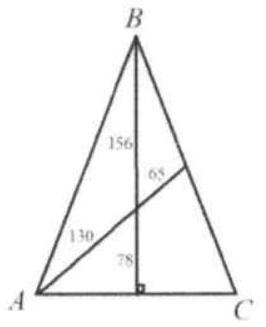
\includegraphics[width=\textwidth]{images/010(1).jpg}\\
\(A F, C E\), and \(B D\) are three medians. They meet at \(G\).\\
\(G D=\frac{1}{3} B D=\frac{1}{3} \times 234=78 . A G=\frac{2}{3} A F=\frac{2}{3} \times 195=130\).\\
Triangle \(A D G\) is a 3-4-5 right triangle \((3 \times 26,4 \times 26,5 \times 26)\) and \(A D=104\).\\
\(S_{\triangle A D G}=\frac{78 \times 104}{2}=4056\)\\
\centering
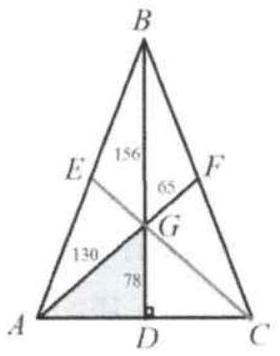
\includegraphics[width=\textwidth]{images/010.jpg}\\
\(S_{\triangle A B C}=6 S_{\triangle A D G}=6 \times 4056=24336\).\\

\end{document}
